\chapter{Methods and results}
\label{chap:problemsolving}

\startcontents[chapters]
\printmyminitoc{
}

\section{Fiber distribution point images processing}

\subsection{Example of forgery cases}

Multiple types of forgery images have been discovered. The method of detection should detect the forgery of these cases. The way these images are retouched includes:

\begin{itemize}
    \item Slightly rotate the image
    \item Add into the image a color bar or put it inside a color box.
    \item Cropped
    \item Color shift.
\end{itemize}


\begin{figure}[H]
    \centering
    \begin{subfigure}{0.4\textwidth}
        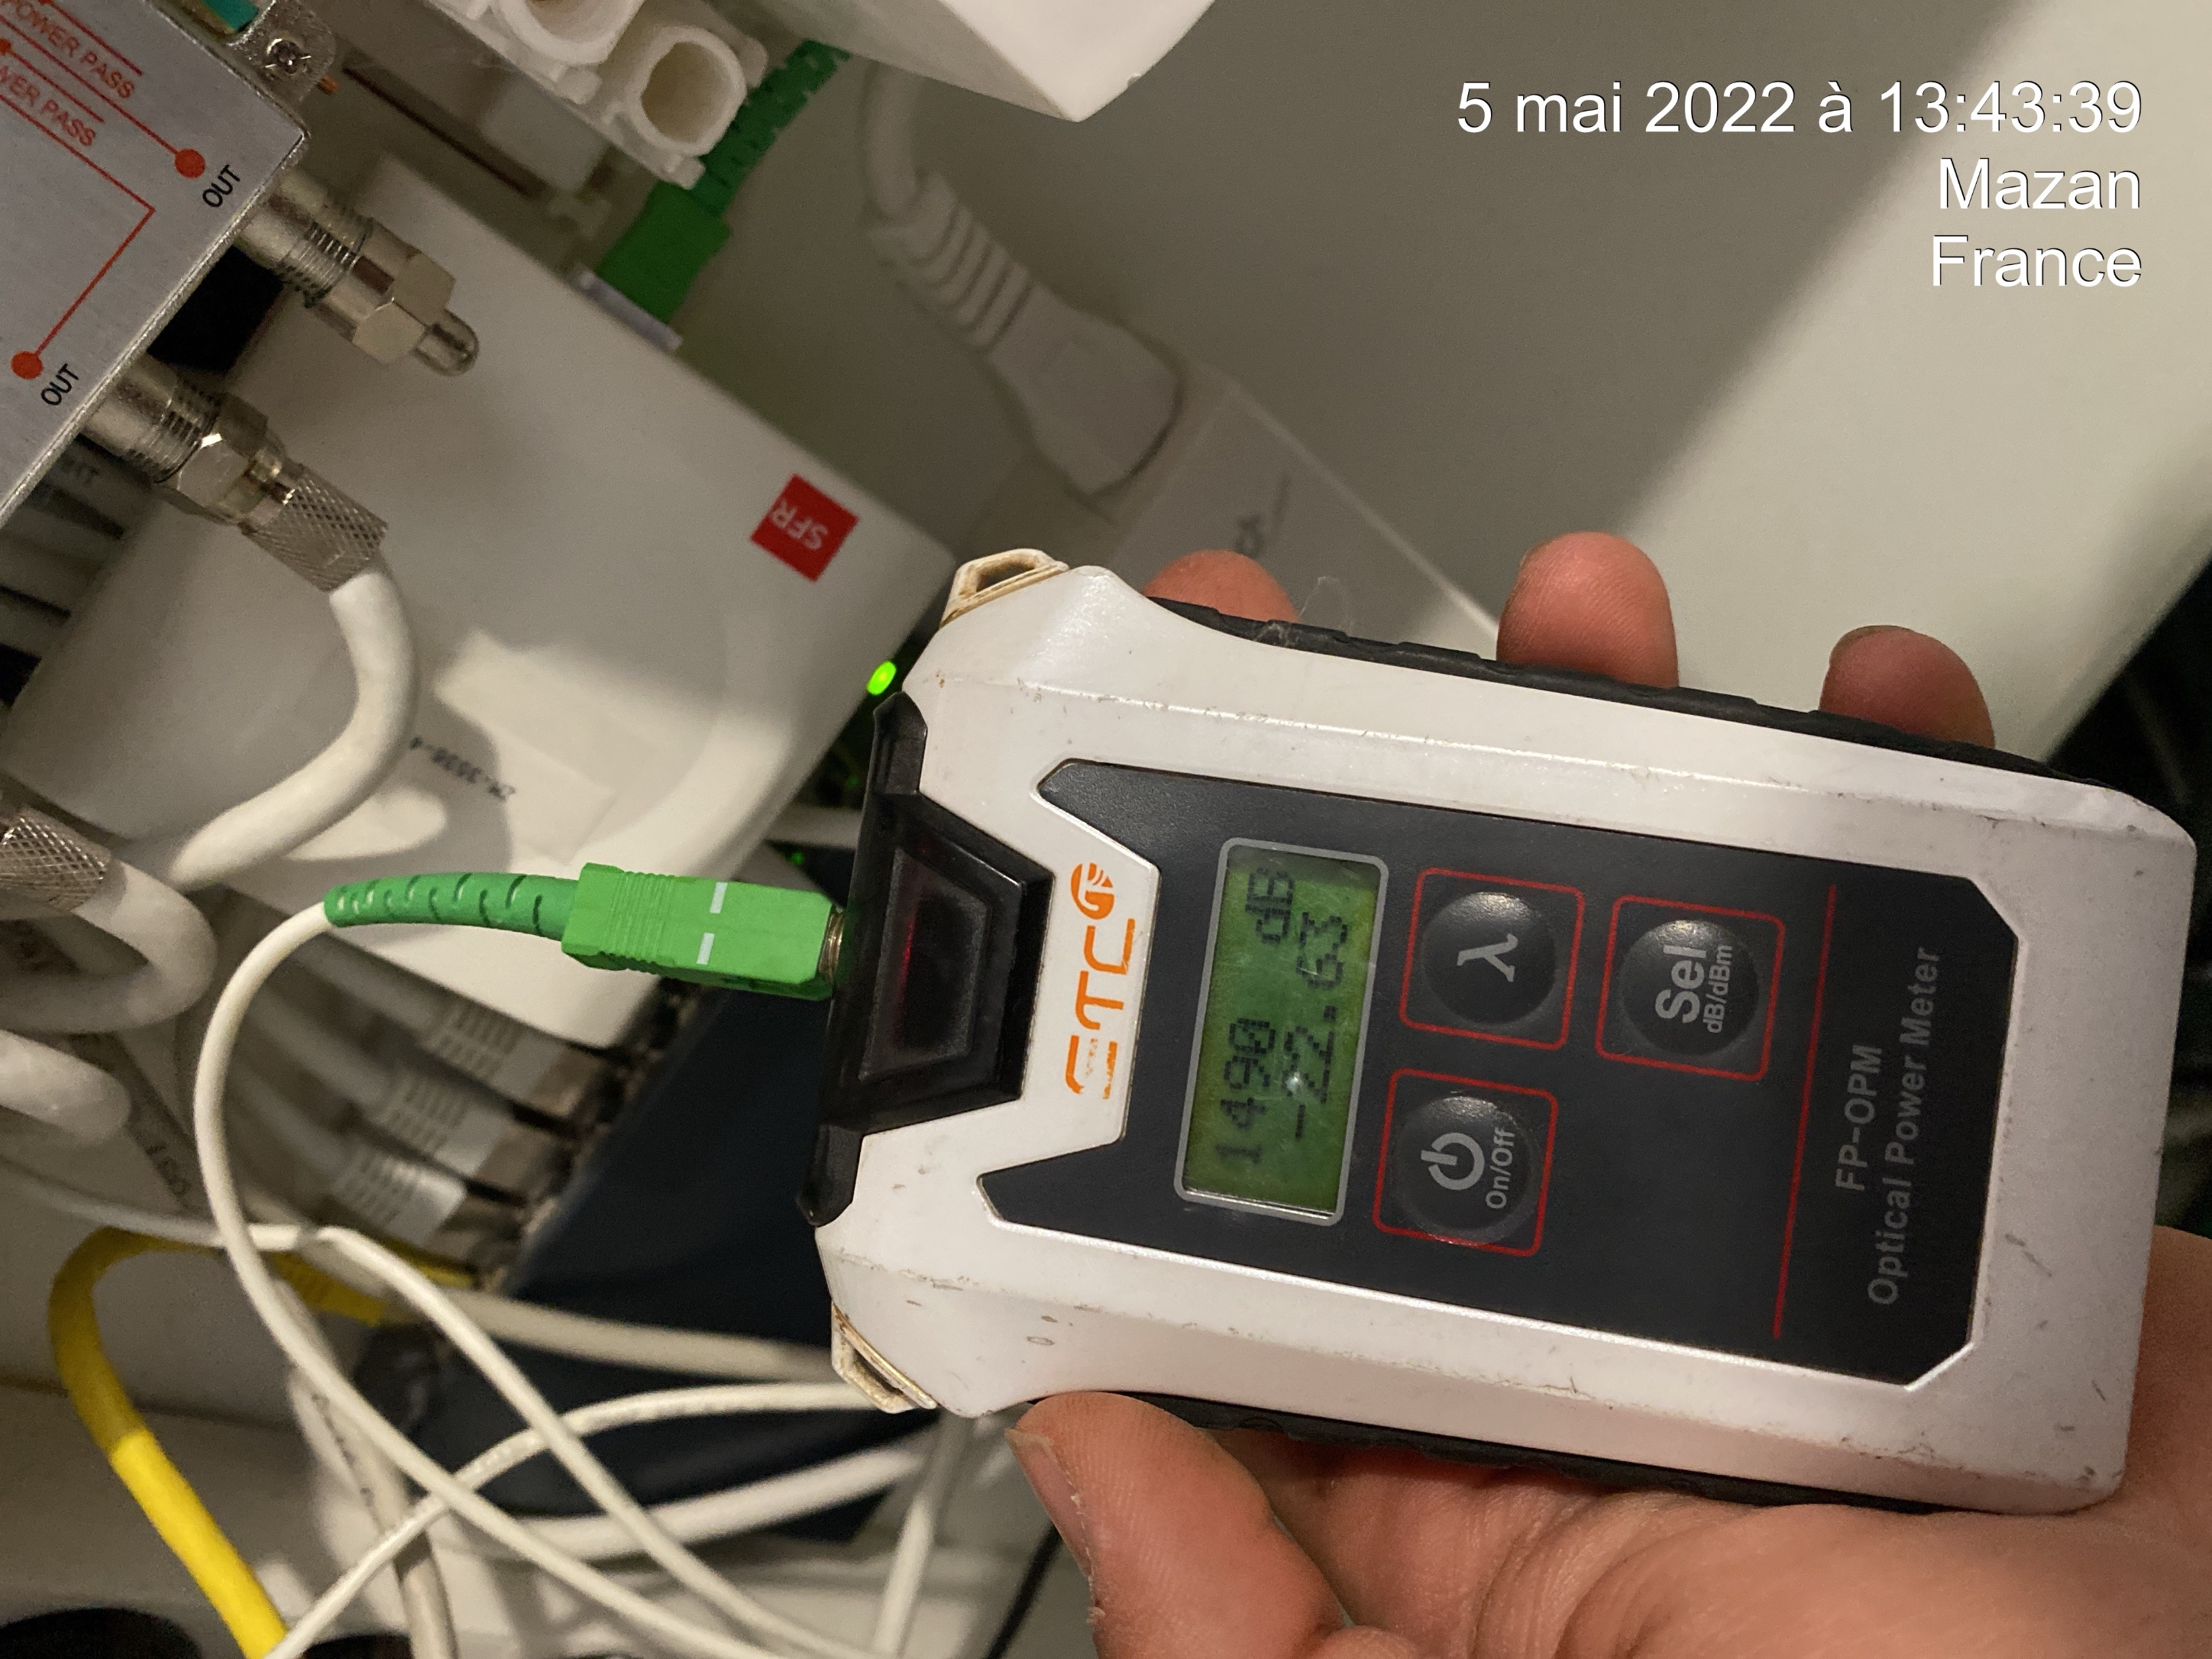
\includegraphics[width=\linewidth]{images/true_positif/t1_true_positif.jpg}
        \caption{Original image}
        \label{fig:true_positif_1}
    \end{subfigure}
    \begin{subfigure}{0.4\textwidth}
        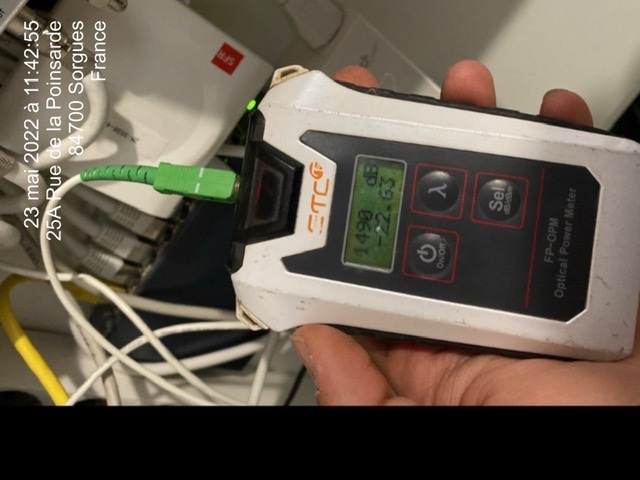
\includegraphics[width=\linewidth]{images/true_positif/t2_true_positif.jpg}
        \caption{Forgery image}
        \label{fig:true_positif_2}
    \end{subfigure}
\end{figure}

As you can see from the example above, the fake image has been cropped a small part at the right side, and then a black bar has been added at the bottom. However, it is also necessary to avoid false alarms. There are a lot of fiber distribution points(PM) that need multiple maintenance. We want to avoid the pictures of the same PM but on different days.

\begin{figure}[H]
    \centering
    \begin{subfigure}{0.3\textwidth}
        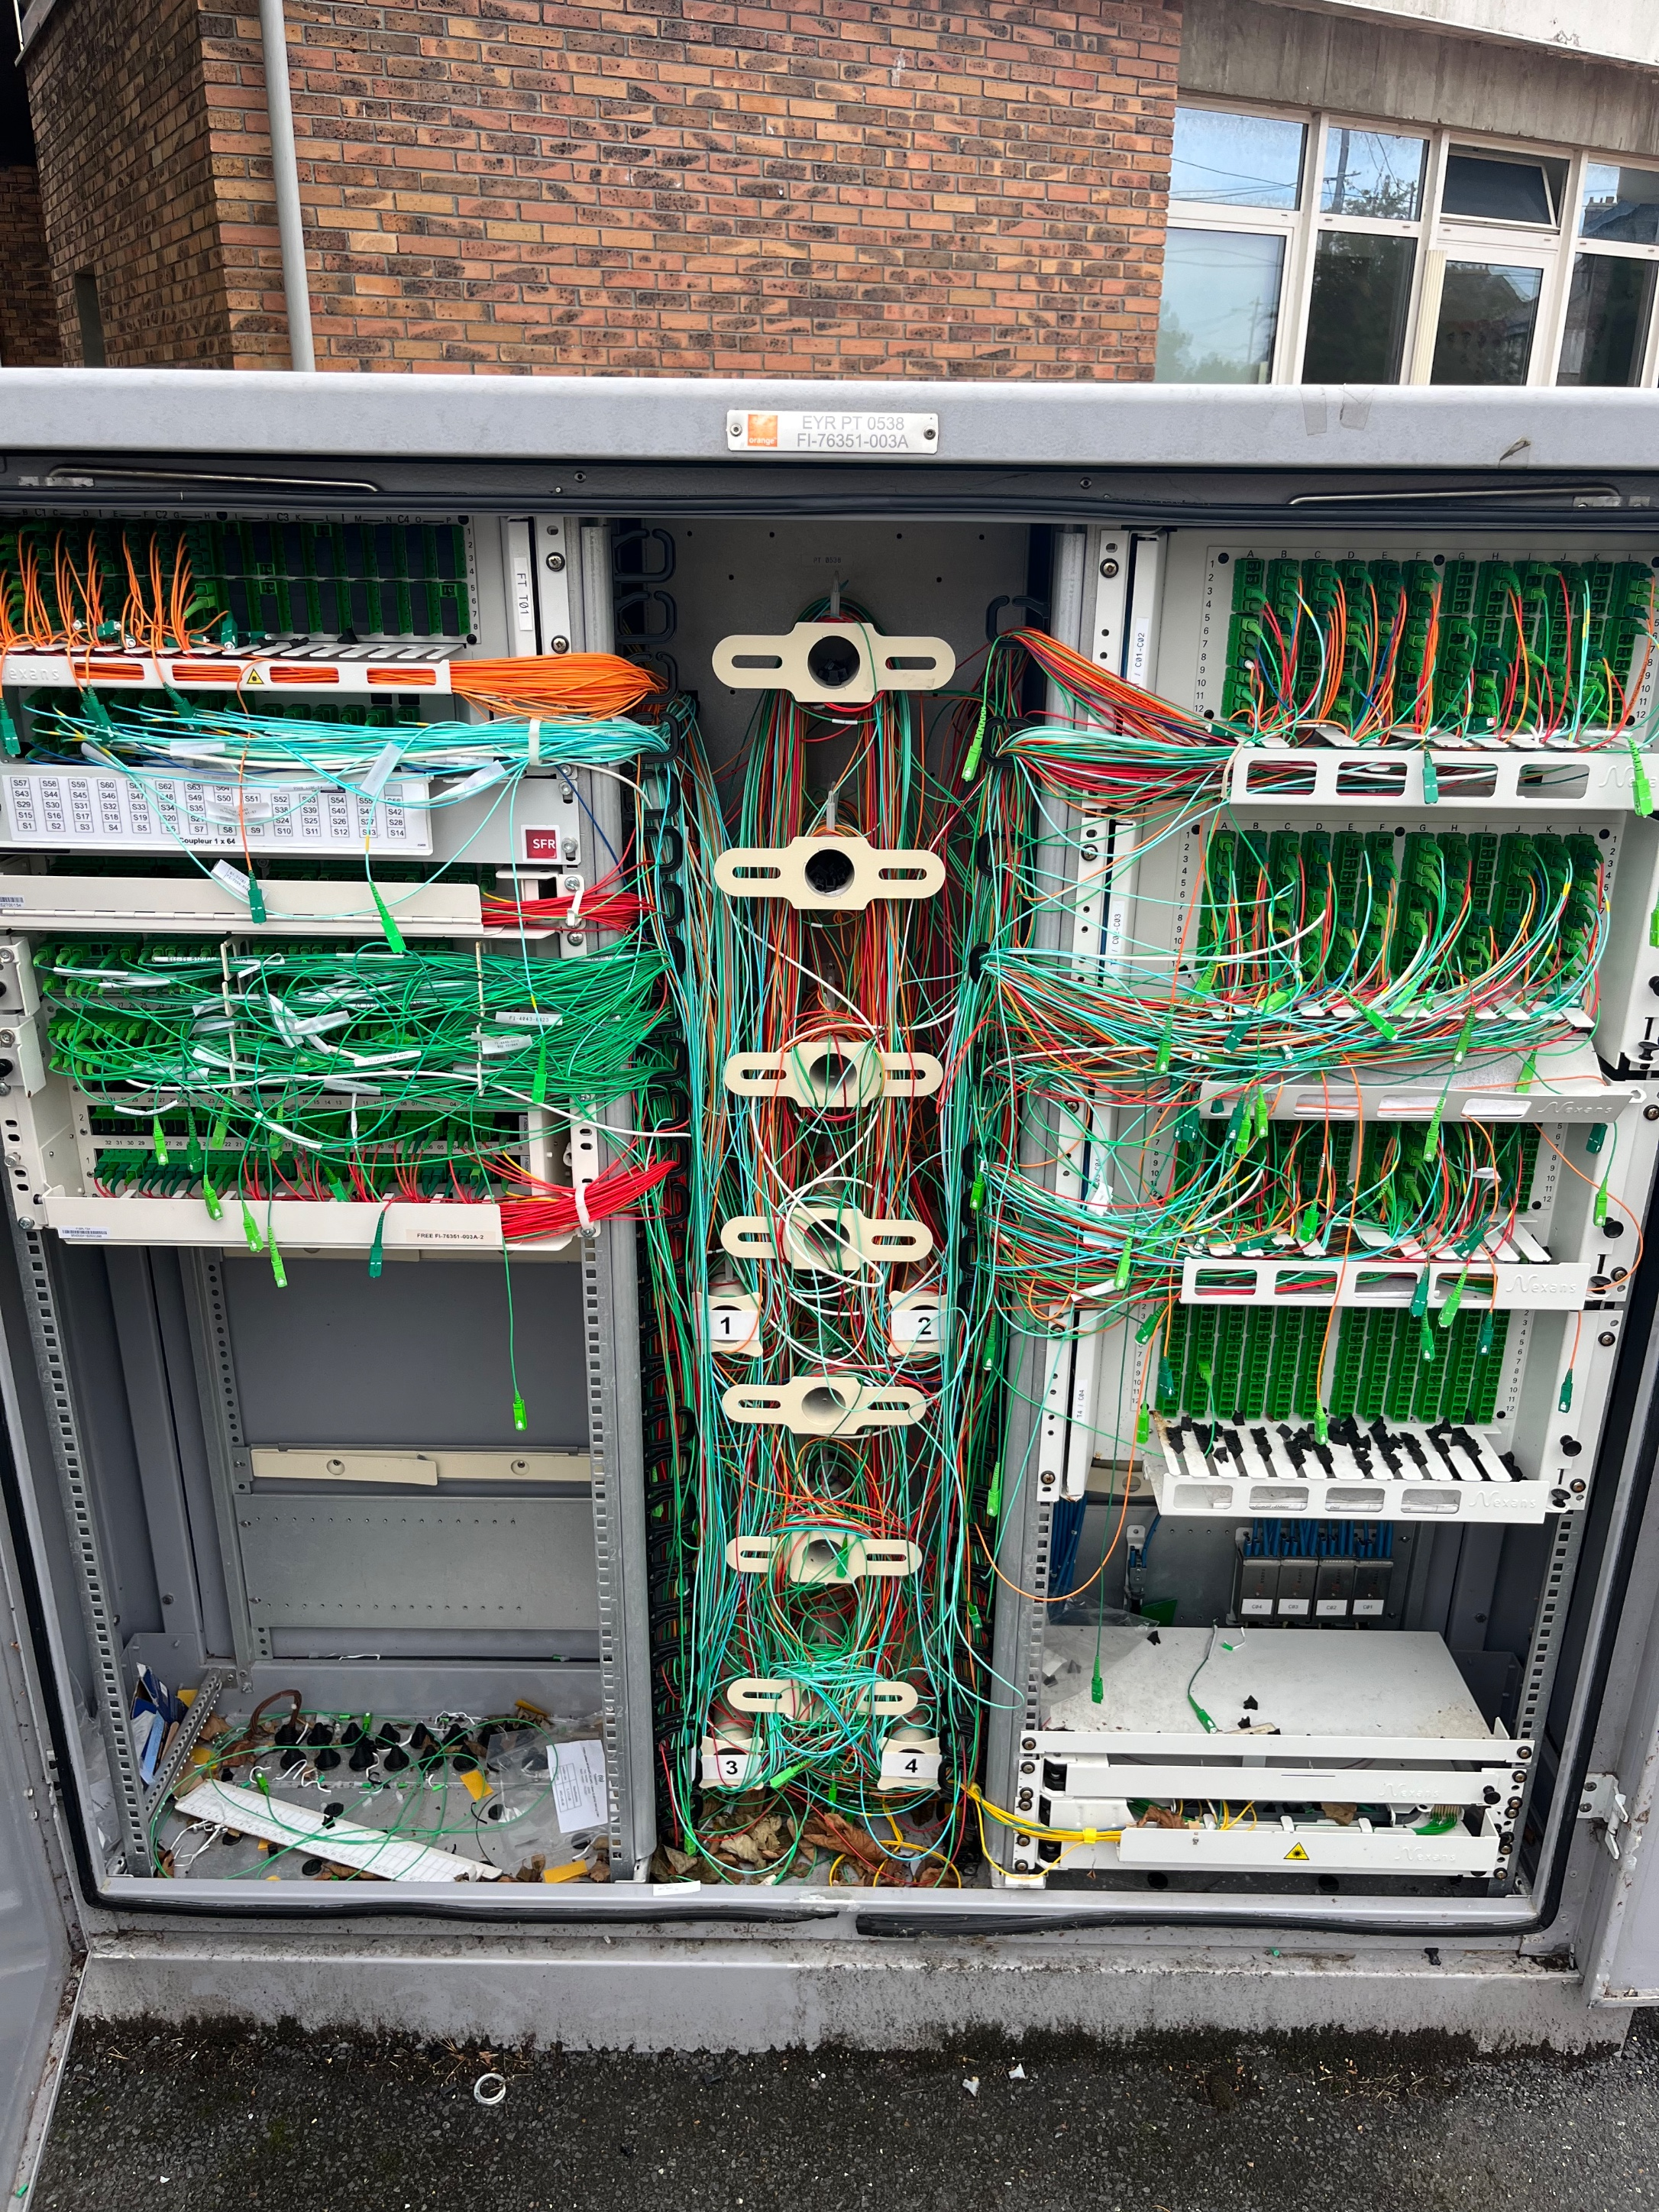
\includegraphics[width=\linewidth]{images/false_positif/5173534_1.jpg}
        \caption{Example of a false alarm - 1}
    \end{subfigure}
    \begin{subfigure}{0.3\textwidth}
        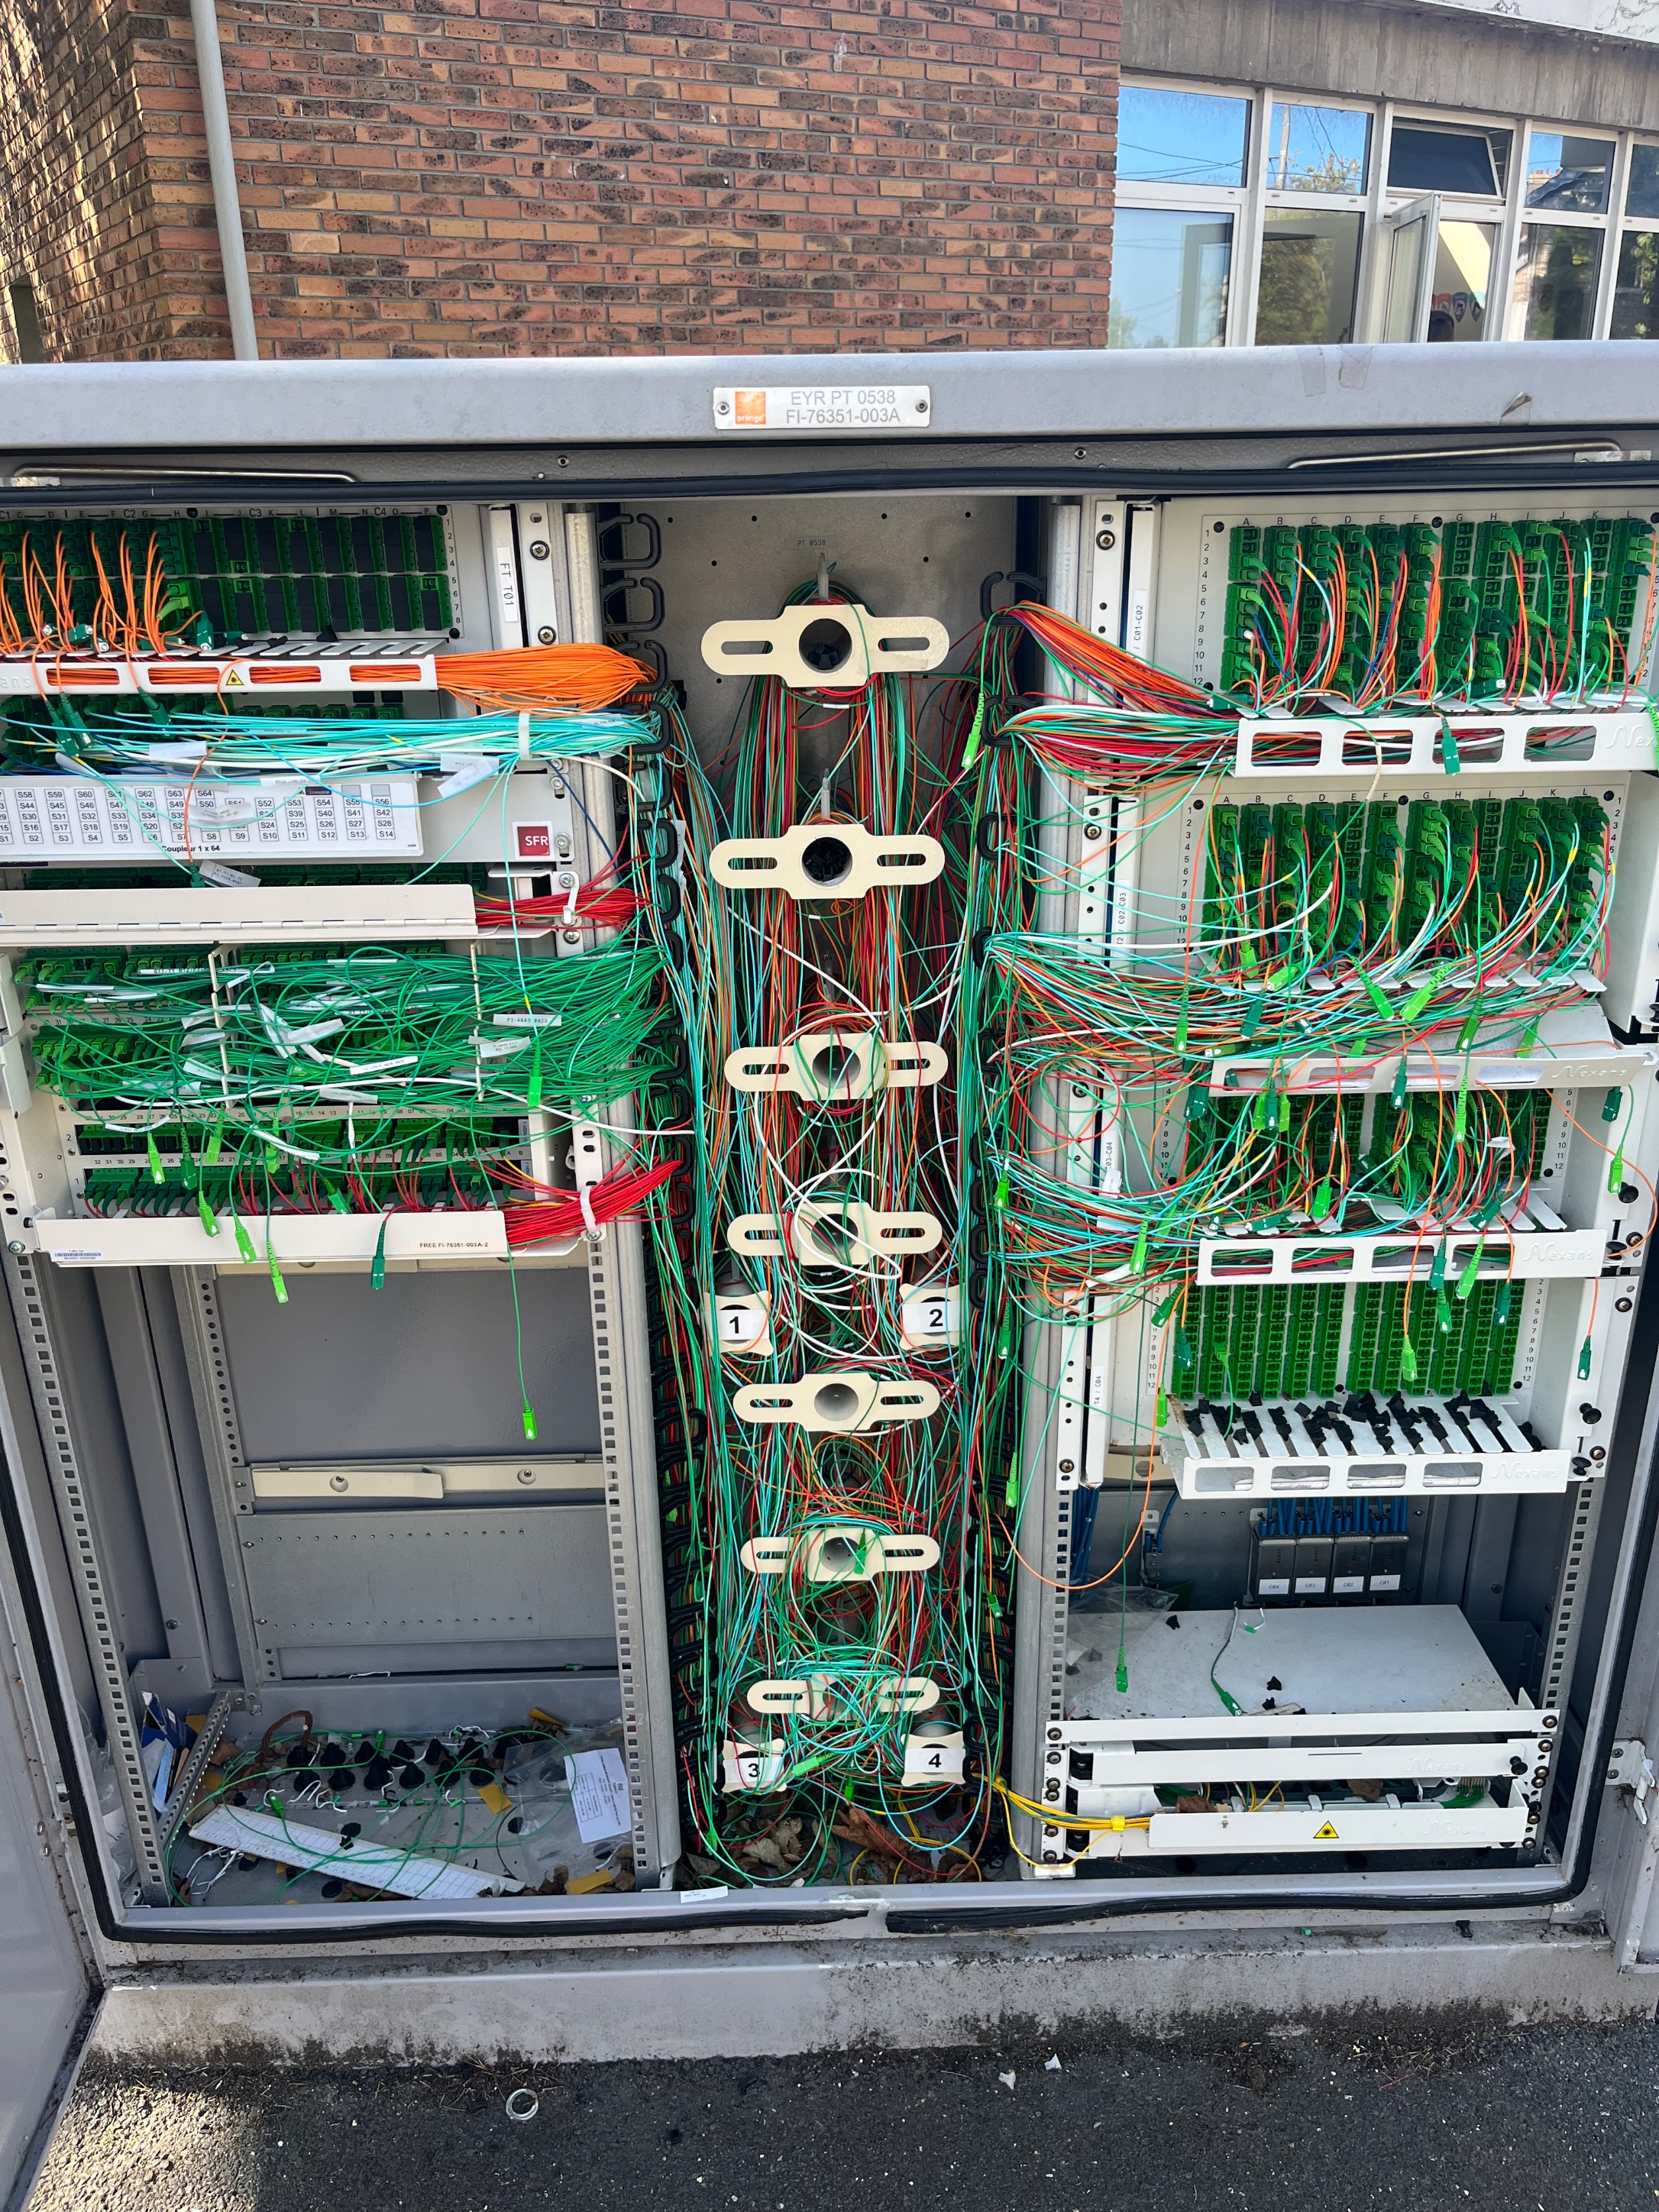
\includegraphics[width=\linewidth]{images/false_positif/5173534_2.jpg}
        \caption{Example of a false alarm - 2}
    \end{subfigure}
\end{figure}

In this case, these 2 images have been captured on different days of the year. It could be noticed when to notice the lighting of the image under the left PM door. In the second image, there was sunlight in the ground around the PM and the first, there was not.

\begin{figure}[H]
    \centering
    \begin{subfigure}{0.4\textwidth}
        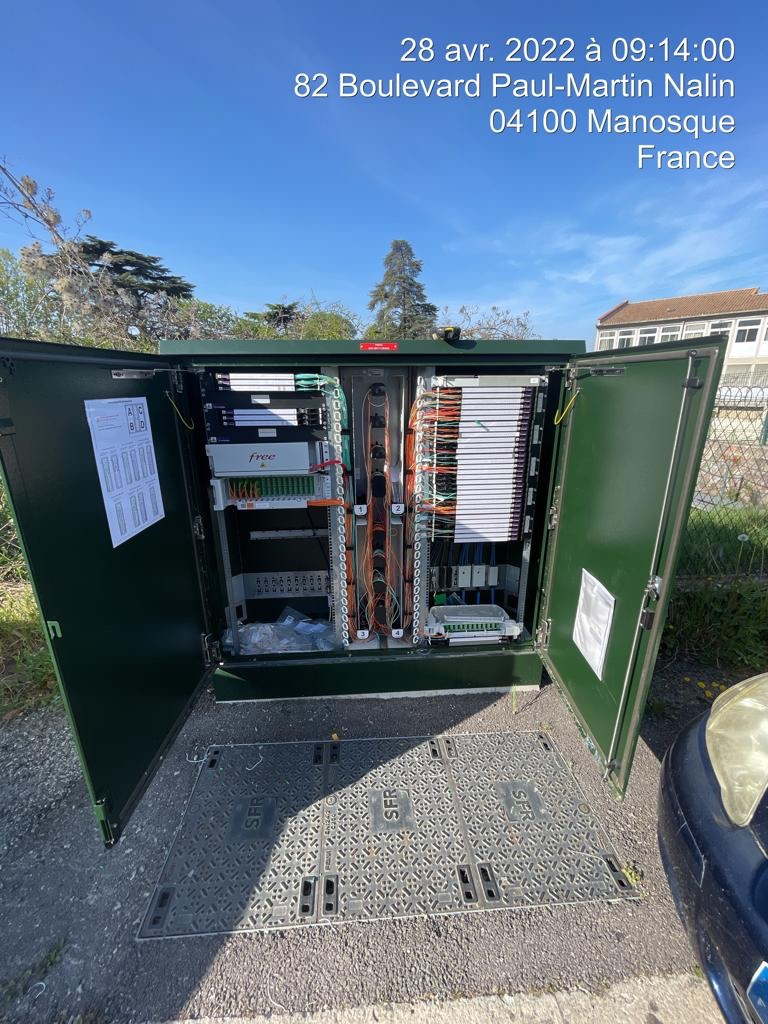
\includegraphics[width=\linewidth]{images/false_positif/f3_1.jpg}
        \caption{Example of a false alarm - 1}
    \end{subfigure}
    \begin{subfigure}{0.4\textwidth}
        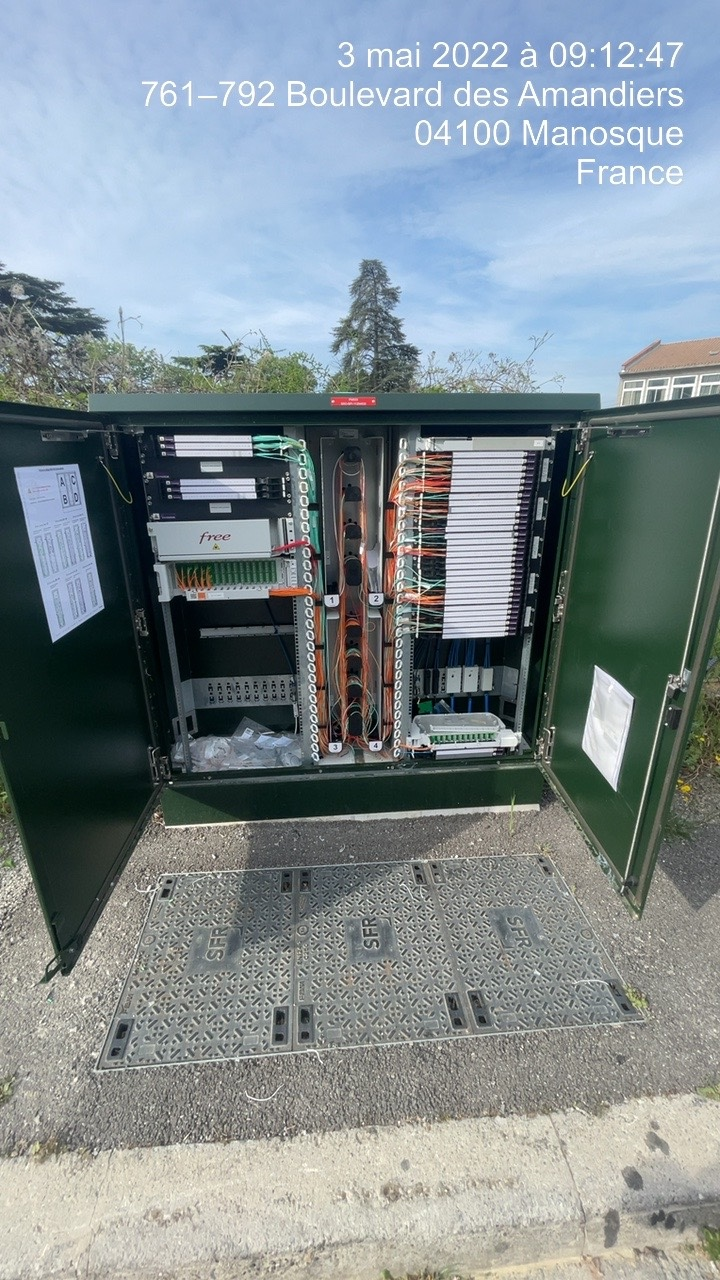
\includegraphics[width=\linewidth]{images/false_positif/f3_2.jpg}
        \caption{Example of a false alarm - 2}
    \end{subfigure}
\end{figure}

In this case, the sky was different because it was on different days. There was also a head of a car on the right of the image in the second image.

\subsection{Method}

This is the overview of the method to compare the similarity between images. The input is the combination of 2 images. The image that is already exists on the database called the \textbf{map} image. The image that it is recently appears that we need to check if forgery is called the \textbf{template} image.

\begin{figure}[H]
    \centering
    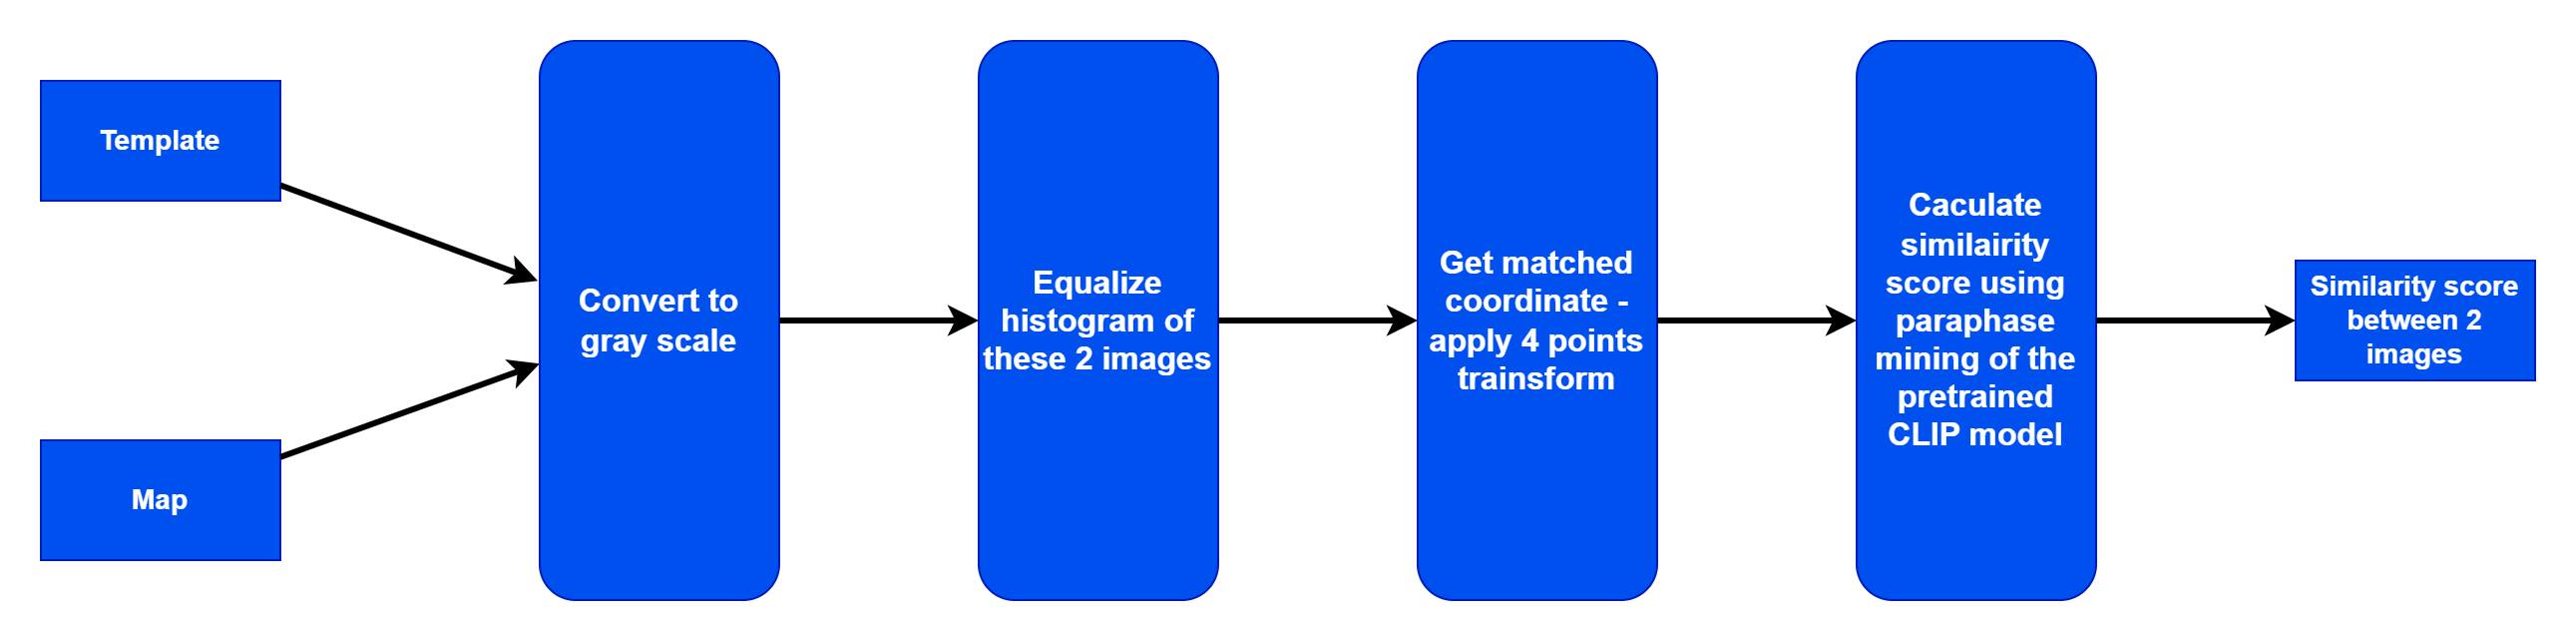
\includegraphics[width=1\textwidth]{images/pm_describe.drawio.png}
    \caption{Overall architecture of the forgery detection system}
    \label{fig:altice_campus}
\end{figure}

\begin{itemize}
    \item \textbf{Convert to grayscale}
    
First, to deal with the problems of color shifting in some of the forgery cases, we need to convert both the map and the template to grayscale images.

    \item \textbf{Equalize histogram}

Even the shift of the lighting image is also important to this task. I use the OpenCV\cite{opencv_library} equalizeHist() function to equalize the histogram of the image before proceeding to the next image.

    \item \textbf{Four points transform}

The scale-invariant feature transform (SIFT)\cite{lowe1999object} is a computer vision algorithm to detect, describe, and match local features in images. Applications include object recognition, robotic mapping and navigation, image stitching, 3D modeling, gesture recognition, video tracking, individual identification of wildlife and match moving.

In this case, I use SIFT to detect the common feature between 2 images and then map the common feature between them. Once the number of matched features exceeds the set threshold, we could use OpenCV homography to correct the point of view of the template to the map.

\begin{figure}[H]
    \centering
    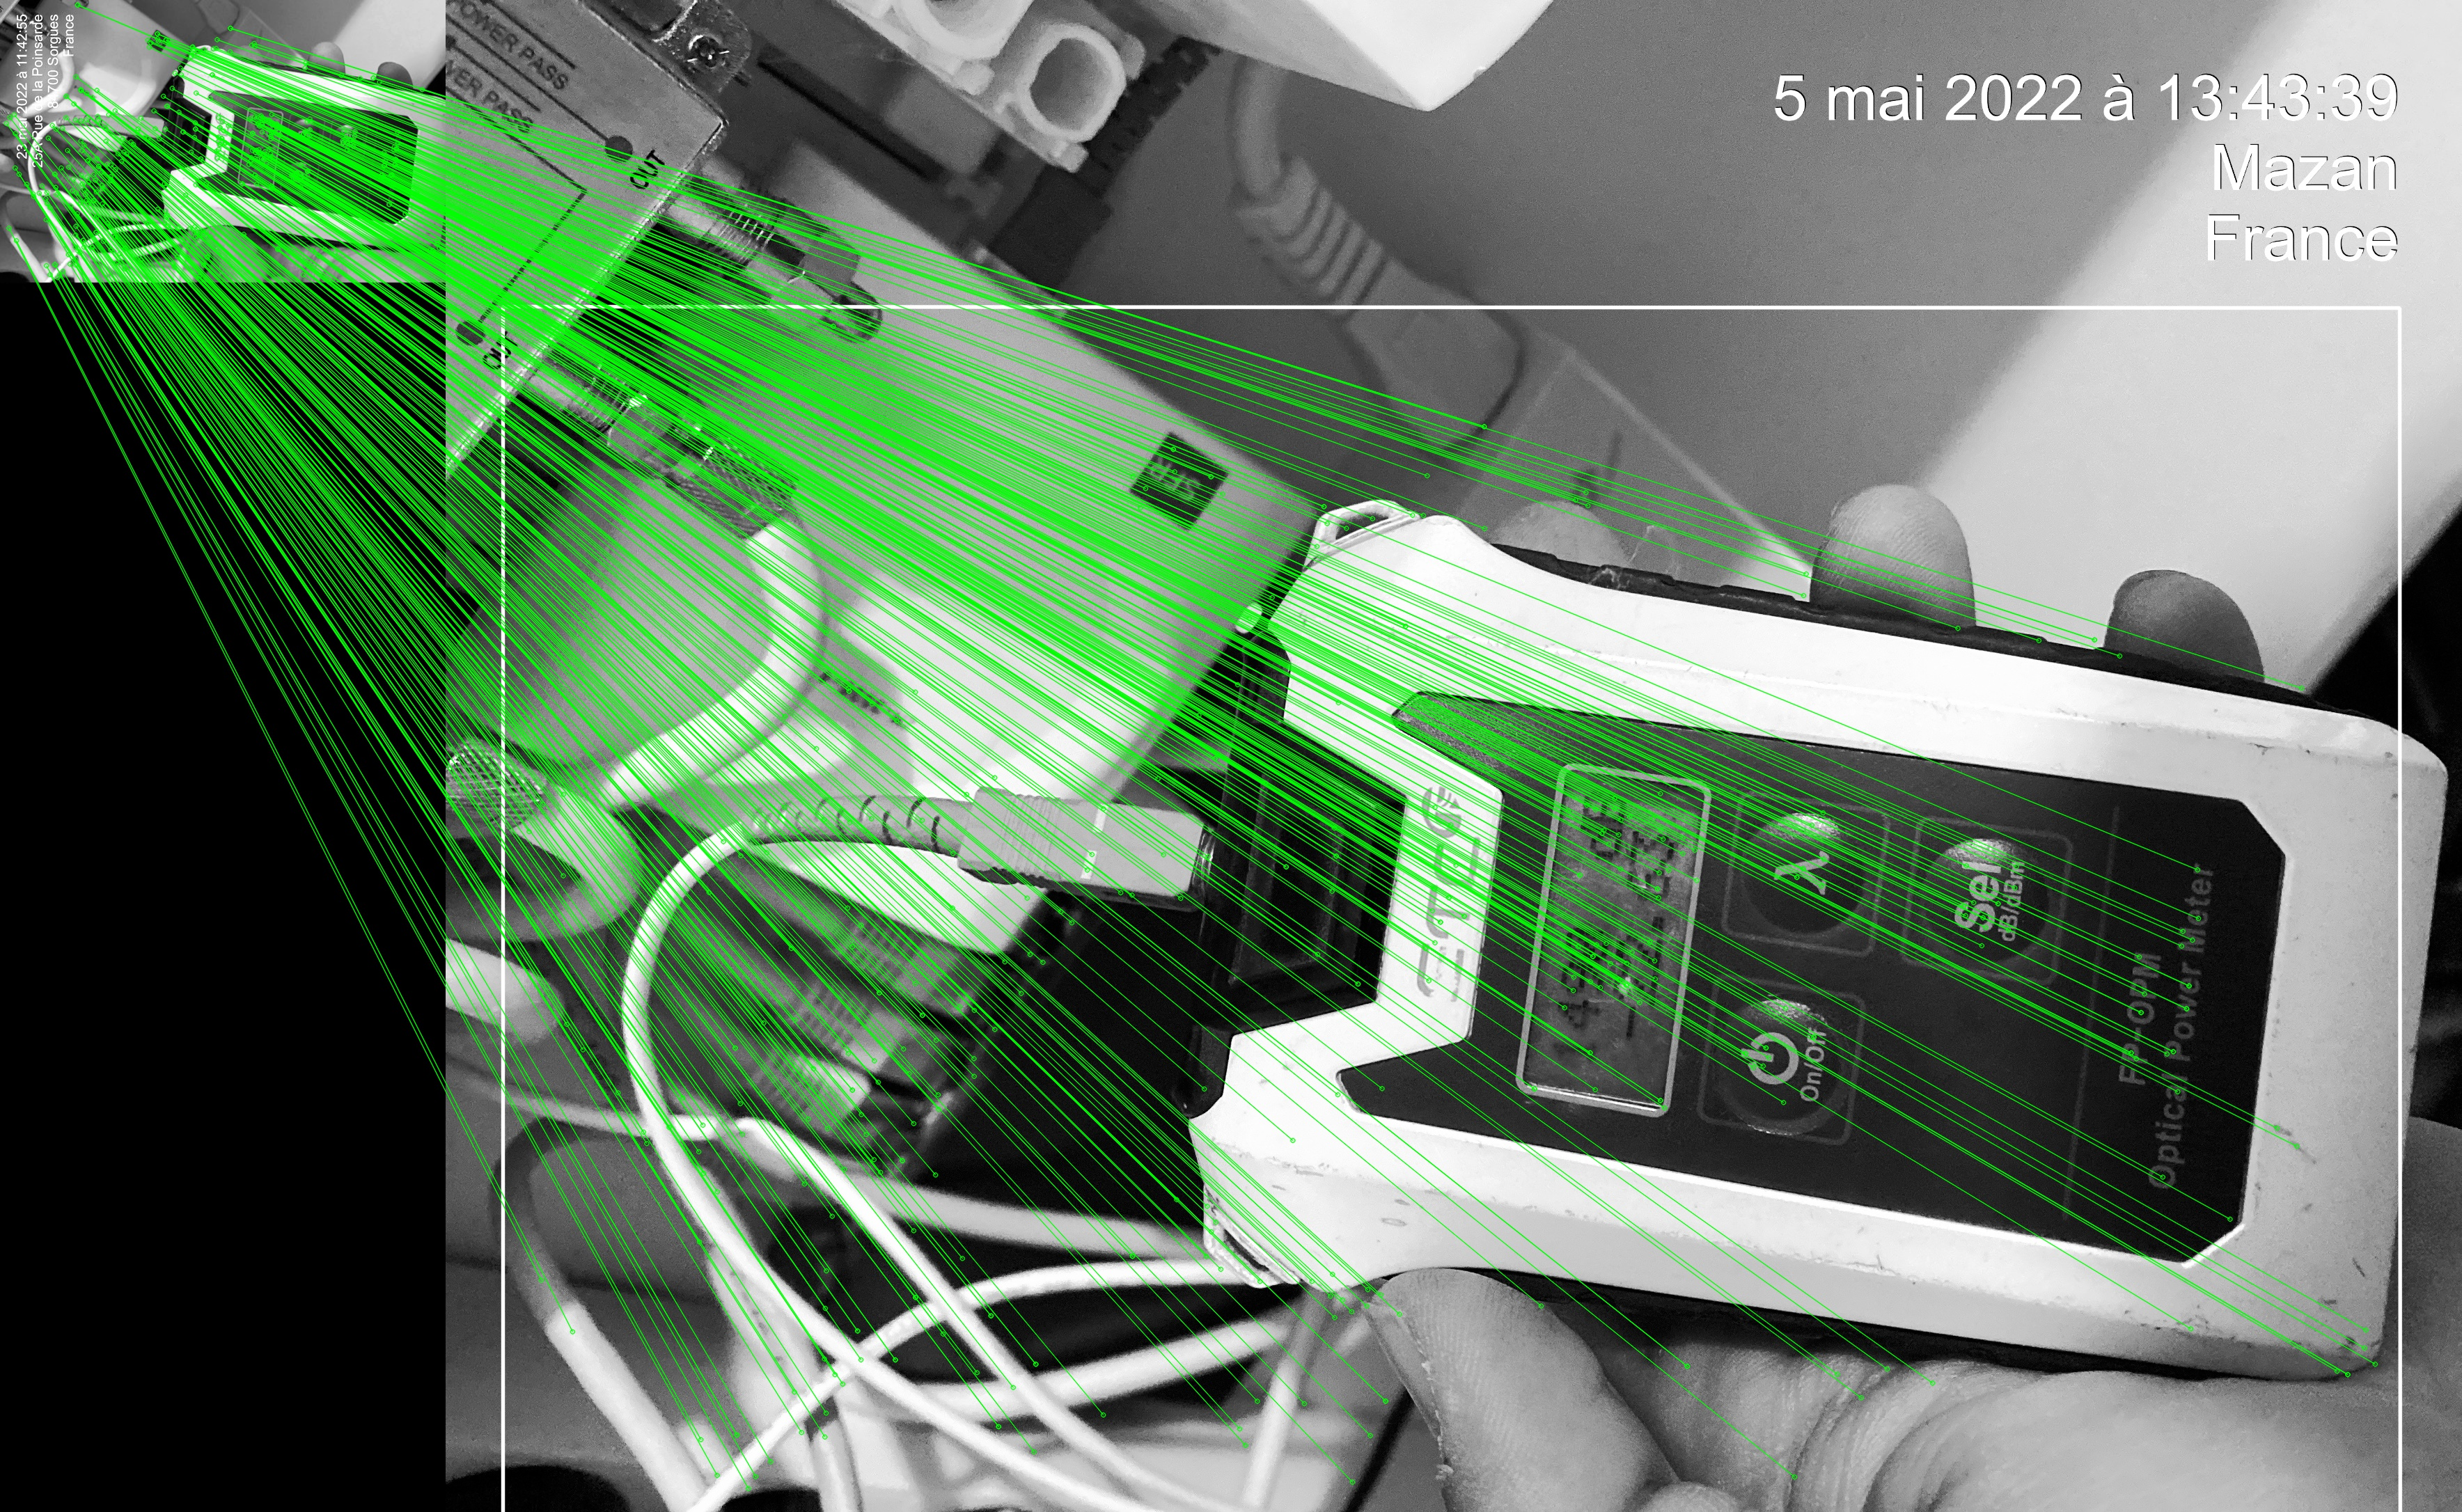
\includegraphics[width=0.8\textwidth]{images/example_front.jpg}
    \caption{Using SIFT and homography to find the coordinate from the template to the map}
    \label{fig:sift}
\end{figure}

The next critical step is to transform the four-point coordinates of the image into a rectangle, like a bird's eye view. We need to do this in the case of detecting images that have been slightly rotated.
    
    \item \textbf{Represent the images to vectors using Contrastive Language-Image Pre-Training (CLIP) model}

In this step, the template has been cropped and transformed to have the same view as the map. So we will be able to avoid retouched elements before we use CLIP\cite{pmlr-v139-radford21a} to calculate the representation vector of the image, thus hoping false alarm cases like the example in 3.1.1 do not affect the representation.
    
\end{itemize}

\subsection{Results}

Due to the lack of labels and lack of true positive cases, I need to create more of the dataset myself by capturing images inside the SFR campus. I captured 2 images of the same place at different times and different angles and created a forgery myself using one of the images with the same forgery techniques that technicians use.

\begin{itemize}
    \item image 1: Original image
    \item image 2: Capture the same place but at a different time and angle
    \item image 1 forgery: a modified version of image 1
\end{itemize}

The dataset used to test this method has been carefully labeled manually, both captured by myself and detected real cases. The score is from 0\% to 100\%, with the higher the score, the most lookalike between 2 images and 100\% is identical.

\begin{figure}[H]
    \centering
    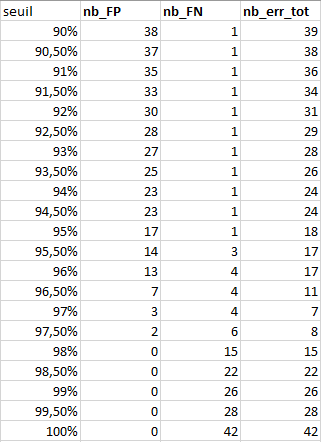
\includegraphics[width=0.5\textwidth]{images/cas_2_confusion_matrix.png}
    \caption{Table of the number of errors by choosing different thresholds of similarity}
    \label{fig:clip_threshold}
\end{figure}


\begin{table}[H]
\centering
\captionof{table}{Threshold table description} \label{tab:description_threshold} 
\begin{tabular}{|l|l|}
\hline
\textbf{column name}  & \textbf{description}              \\ \hline
seuil        & similarity threshold     \\ \hline
nb\_FP       & number of false positive \\ \hline
nb\_FN       & number of false negative \\ \hline
nb\_err\_tot & total number of error    \\ \hline
\end{tabular}
\end{table}

\begin{figure}[H]
    \centering
    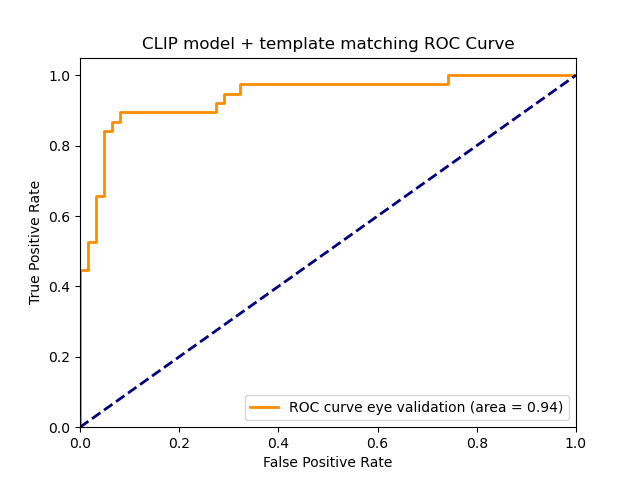
\includegraphics[width=0.8\textwidth]{images/cas_1_roc-curve.png}
    \caption{ROC curve of the method}
    \label{fig:clip_roc-curve}
\end{figure}

As the results show, the best threshold to choose is around 97\% of similarity between the template and the map. Above this score, it is usually forgery cases and below this is false alarm cases.

\section{Research the feasibility of moving the team's infrastructure to the Google Cloud}

\subsection{Example of needed cases}

SFR is an operator in France responsible for managing and maintaining a network of mobile signal towers. Your goal is to ensure uninterrupted mobile signal and internet services for your customers while minimizing downtime and troubleshooting issues efficiently.

Ensuring consistent network performance is challenging due to the complexity of signal tower operations and the potential for various issues such as hardware failures, signal interference, and congestion. We want to implement a system that can detect anomalies in real-time and help us address them before they impact customer experience.

\subsection{Use case of VertexAI}

\begin{itemize}
    \item \textbf{Data Collection and Integration:}
    
    Data is collected from multiple sources within the network, including signal strength measurements, network traffic data, tower hardware status, and historical performance data.
    \item \textbf{Model Development:}

    Machine learning models for anomaly detection are developed using Vertex AI's capabilities. These models are trained on historical data to learn normal patterns of network behavior.

    \item \textbf{Real-time Anomaly Detection:}

    Deployed models continuously monitor incoming data from signal towers in real-time.
    Deviations from expected patterns trigger alerts, notifying network operators of potential anomalies.

    \item \textbf{Alert Prioritization and Response:}

    Generated alerts are prioritized based on severity and potential impact on network performance. Vertex AI's insights assist in identifying root causes and appropriate responses.

    \item \textbf{Continuous Improvement:}

    Feedback loops are established to refine models based on accuracy and response effectiveness. Collaboration with data scientists fine-tune models for improved anomaly detection.

    \item \textbf{Performance Monitoring:}

    Vertex AI's visualization tools track the overall performance of the anomaly detection system. Key metrics, including detected anomalies, false positives, and response times, are monitored.
\end{itemize}




\section{Apply machine learning techniques on call log from SFR's call center}

The below diagram shows the overall architecture of the system. We want to try to benefit the representation of the language model in this use case of finding the topics in the corpus of the company's call center.

\begin{figure}[H]
    \centering
    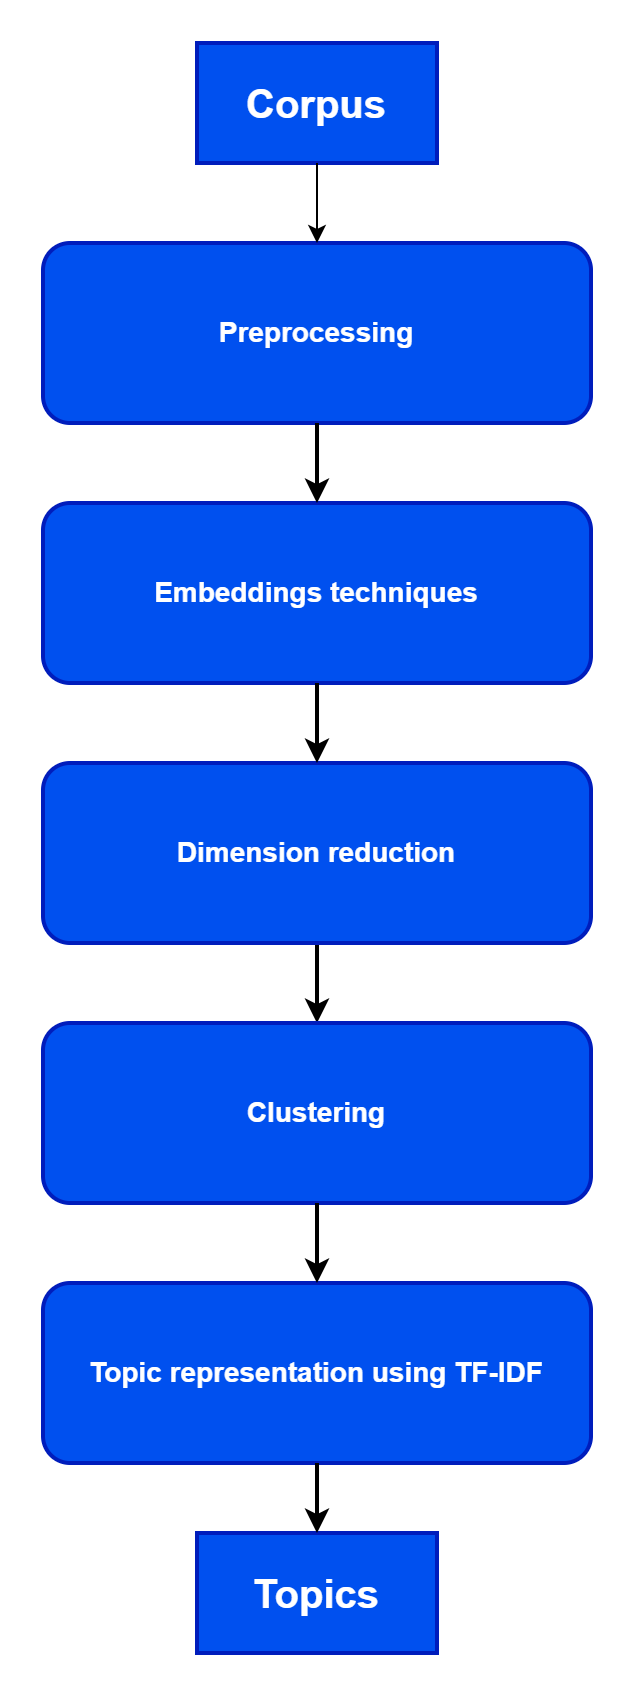
\includegraphics[width=0.4\textwidth]{images/describe_nlp.drawio.png}
    \caption{Algorithm description}
    \label{fig:nlp_describe}
\end{figure}

The process starts with preprocessing, which turns the given dataset into the form that is needed for the embedding techniques. Some soft clean is also applied to the corpus before translating the sentence into vectors. After we have the desired corpus, it will be represented as a vector in a fined vector space with the help of a sentence transformer. The dimension reduction techniques are then applied, and we use the output of the process as data points to do the main task of clustering. After that, we use a special version of TF-IDF to find the most significant word of each found topic.

This project will be kept as the topic for the memoir, I will go into further detail in the memoir section. This part will introduce briefly the overall architecture.

The output of this project is the list of significant words and the input is the new conversation with the customer that was also introduced to the system.

\begin{figure}[H]
    \centering
    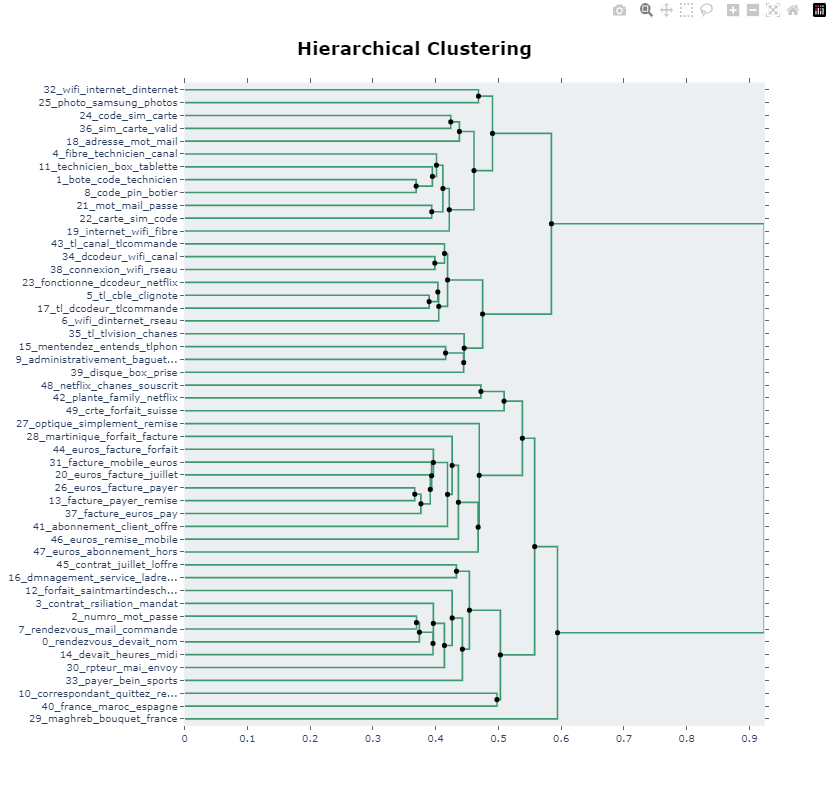
\includegraphics[width=1\textwidth]{images/results/cam/hierachy_pca_tree.png}
    \caption{One of the results using hierarchy clustering and PCA}
    \label{fig:hierachy_pca}
\end{figure}
